\documentclass[a4paper, 11pt] {article}
\usepackage[margin=2cm]{geometry}
\usepackage{placeins}
\usepackage{Float}
\usepackage{graphicx}
\usepackage{wrapfig}
\graphicspath{{/.}}
\begin{document}
\title{ECM2414 Card Game Coursework}
\author{690037391 \& 680039372}
\date{\today}
\maketitle
	\begin{center}
		Marks Split: 50:50
	\end{center}
\pagebreak
\section*{Development Log}
\begin{center}
\begin{table}[H]
\begin{tabular}{|l|l|l|l|l|}
\hline
Date           & Time     & Duration  & Roles                                                 & Signature                       \\ \hline
 26/10/2020 & 11:30    & 1hr 40m  & Driver: 680039372, Navigator: 690037391 & 680039372 \& 690037391 \\ \hline
 26/10/2020 & 13:20    & 1hr 40m  & Driver: 690037391, Navigator: 680039372 & 680039372 \& 690037391 \\ \hline
 26/10/2020 & 15:00    & 2hr 00m & Driver: 680039372, Navigator: 690037391 & 680039372 \& 690037391 \\ \hline
 27/10/2020 & 11:30    & 2hr 00m & Driver: 690037391, Navigator: 680039372 & 680039372 \& 690037391 \\ \hline
 27/10/2020 & 13:30 & 2hr 00m & Driver: 680039372, Navigator: 690037391 & 680039372 \& 690037391 \\ \hline
 28/10/2020 & 11:30 & 1hr 30m & Driver: 690037391, Navigator: 680039372 & 680039372 \& 690037391 \\ \hline
\end{tabular}
\end{table}
\end{center}
\FloatBarrier
\pagebreak
\section*{Production Code Design}
\subsection*{Preliminary User Input}
The \texttt{CardGame} class will query the user for the initial parameters to setup the game, such as the number of players and the path to the file specifying the cards in the game. Once the system is provided with the correct information, the next phase will start.
\subsubsection*{Number of Player Query}
If the user doesn't enter a valid input (a positive integer), the system should explain that the input is invalid and it should ask the user for the correct input.
\subsubsection*{Pack File Query}
If the user doesn't enter a real path, the system should explain and ask the user to input a real path.
Should a real file be provided, the system should check each line to see if it is a positive integer, and if not, it should explain to the user that the file they provided contains invalid cards. It should then ask the user to provide another path to a valid deck.

Should all the cards in the file be valid, the system then check to see if the amount of cards found is equal to $8n$, $n$ being the number of players in the game. If it has too many or too little cards, the system should explain that to the user and ask for a new file that has the right amount of cards.
\subsection*{\texttt{Player} Class}
The \texttt{Player} class implements the \texttt{Runnable} interface and represents a player as a thread. 
The \texttt{Player} should have a public \texttt{playerNumber} (the number assigned to a player) and a private \texttt{hand} (which is a list of \texttt{Card} instances). 
The \texttt{Player} will have 1 getter method, \texttt{getNumberOfCards()} which returns the number of cards. 
It will also have two action methods, \texttt{addToHand(Card card)} and \texttt{discardCard(Card card)}. The former will add the card to the hand or throw a \texttt{HandFullException} if the hand is full (contains 4 cards). The latter will remove the card from the hand or throw a \texttt{HandEmptyException} if the hand is empty. 
The predicate \texttt{hasWon()} returns a boolean depending on whether a player's hand meets the winning condition. 
The \texttt{takeTurn(CardDeck deckLeft, CardDeck deckRight)} method combines both actions into a single atomic action, wherein a player takes a card from the left, checks if it is preferred and either adds it to their hand if it is or discards the card to their right if it does not. 
Finally, this class overrides the \texttt{Runnable run()} method, implementing a locking system between threads (seen in the \textbf{Locking} subsection).

\subsection*{CardDeck Class}
The \texttt{CardDeck} class has a private final \texttt{deckNumber} (the number assigned to the deck) and an \texttt{ArrayDeque<Card> deck)} which is a Double ended queue of \texttt{Card} objects, allowing for insertion of a card at the end of the queue and taking of a card from the head of the queue. This class also has a getter method (\texttt{getDeckNumber()}) which returns the number of the deck. This class also has an \texttt{addCard(Card card)} and a \texttt{removeCard(Card card)} method which adds a card to the \texttt{deck} queue or remove a card from the \texttt{deck} queue respectively. Finally, this class has a \texttt{takeCard()} method which returns and removes the head of the \texttt{deck} queue, allowing for a player to take a card from the top of a deck.

\subsection*{Card Class}
The \texttt{Card} class represents the cards themselves and has a single \texttt{final int denomination} attribute which represents the integer denomination and has a constructor which sets the \texttt{denomination}.

\subsection*{Locking System}
\begin{wrapfigure}{r}{0.3\textwidth}
\centering
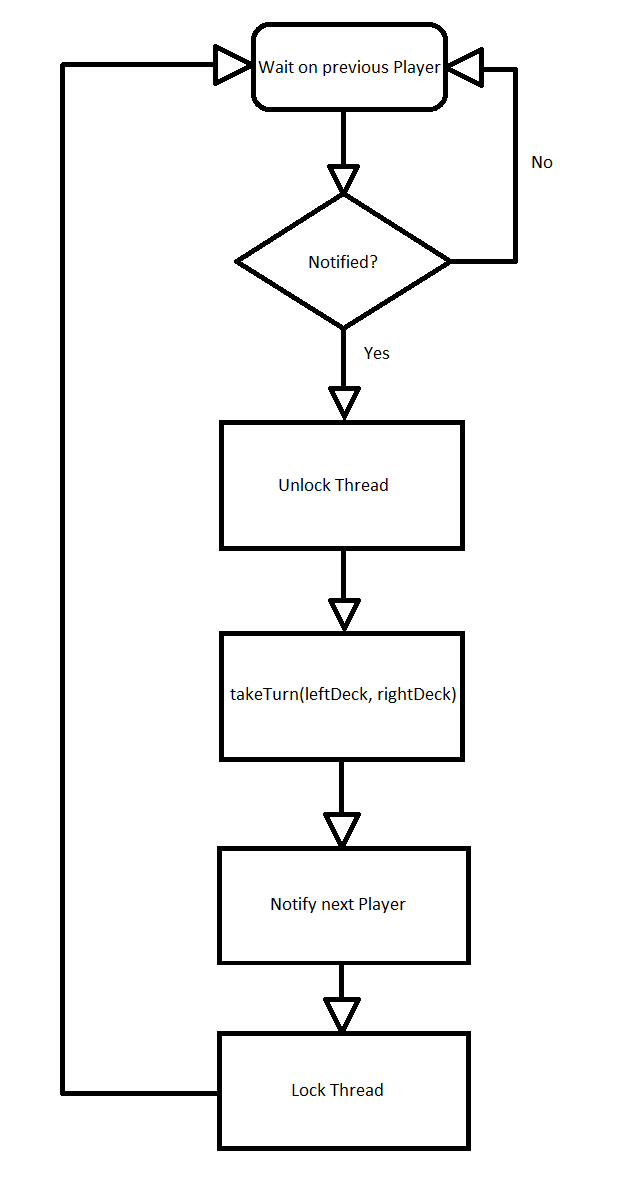
\includegraphics[width=0.3\textwidth]{thread_locking.png}
\end{wrapfigure}

To prevent deadlocking and other concurrency issues, a simple locking system will be put into place. In this system, all \texttt{Player} threads are created, run and then all set to wait on a lock on the previous player in the ring system (i.e. Player 1 waits on Player 4, Player 3 waits on Player 2). The main program thread in which the \texttt{CardGame} main method runs will notify the first Player, who removes their lock and which invokes their \texttt{takeTurn} method; once a player finishes their turn, they proceed to notify the next player in the ring and then lock themselves. This creates a loop around the ring of waiting, unlocking, taking turns, notifying the next player, locking and waiting for the previous player. See to the right a flowchart of the locking system.


\pagebreak
\section*{Testing Design}
\subsection*{Framework}
We are using JUnit 5 for our unit tests and testing suite.

\end{document}